
An oscilloscope is an electronic instrument used to visualize and analyze electrical signals by displaying their voltage waveforms over time. It provides real-time information about the behavior of a signal, enabling users to measure parameters like amplitude, frequency, and waveform shape, which are crucial in various fields like electronics, telecommunications, and research.

\begin{figure}[h!]
    \centering
    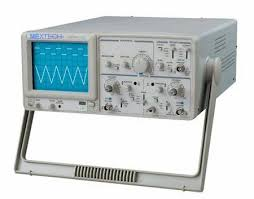
\includegraphics[width=0.4\textwidth]{figures/oscilloscope.jpeg}
    \caption{oscilloscope}
    \label{fig:sample_image}
\end{figure}
 

\subsection{How an Analog oscilloscope works?}
\begin{figure}[h!]
    \centering
    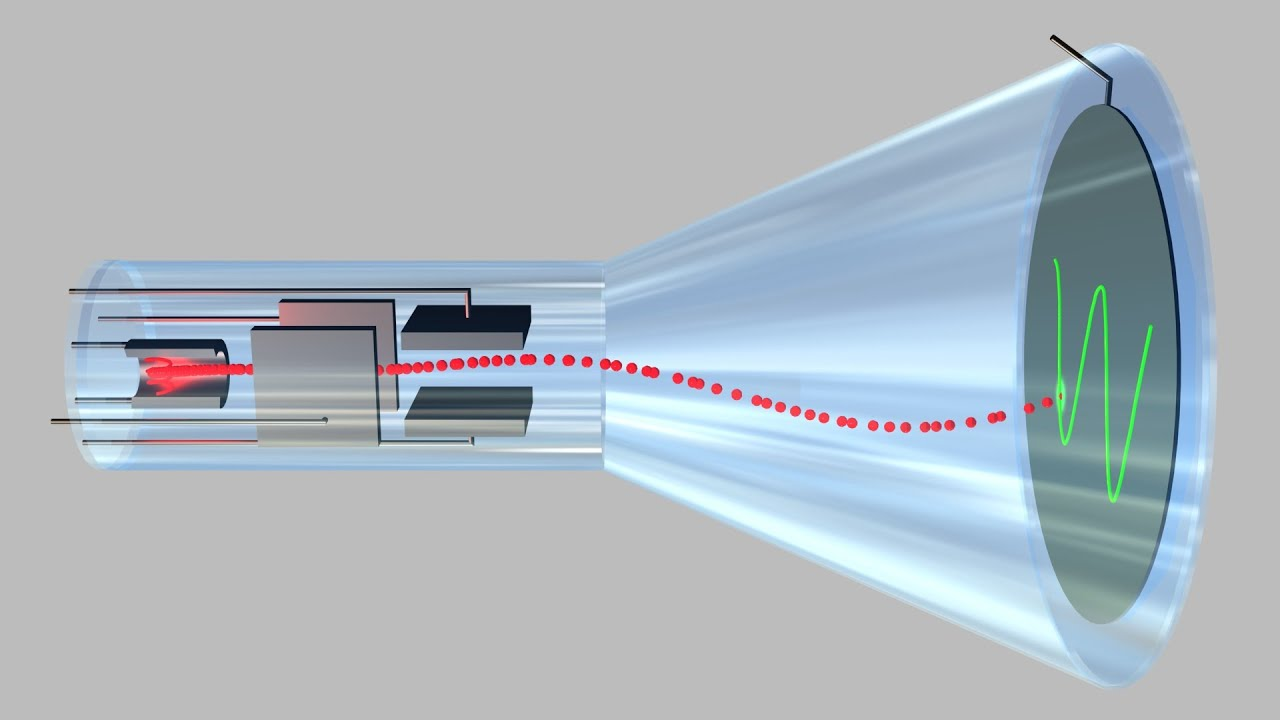
\includegraphics[width=0.4\textwidth]{figures/cathoderay.jpeg}
    \caption{This is a sample image.}
    \label{fig:sample_image}
\end{figure}

An analog oscilloscope uses an electron gun to direct a beam onto a phosphor-coated screen, where voltage waveforms are displayed. The vertical deflection plates control the beam's movement according to the input signal's voltage, and the horizontal deflection plates control the beam's movement based on time. The time base synchronizes the beam's horizontal sweep to ensure stable display. The signal's variations are shown as a trace on the screen, where each division corresponds to specific voltage or time intervals. Triggering ensures the waveform is stable and consistent.
\\

\subsection{How is Digital Oscilloscope Different from Analog Oscilloscope?}

Unlike an analog oscilloscope, a digital oscilloscope converts the analog input signal into digital data using an analog-to-digital converter (ADC). This digital representation is processed and displayed, providing more accuracy, stability, and flexibility. Digital oscilloscopes offer higher resolution, advanced triggering features, and the ability to store and recall waveforms for later analysis. They are generally more versatile, allowing for complex measurements and data manipulation, which makes them superior for detailed analysis compared to analog oscilloscopes.
